\documentclass[a4paper, 12pt, oneside, titlepage]{article} %{\parskip}
\usepackage[top=2.54cm, bottom=2.54cm, left=3cm, right=2cm]{geometry}
\usepackage[utf8]{inputenc}
\usepackage[czech]{babel}
\usepackage[T1]{fontenc}
\usepackage{graphicx}
\usepackage{booktabs}
\usepackage{tabularx}
\usepackage{array}
\usepackage{indentfirst}
\usepackage{multicol}
\usepackage{titlesec}
\usepackage{mathtools}
\usepackage{esvect}

\usepackage{url}
\usepackage{caption}
\usepackage{subfig}
\usepackage[section]{placeins}
\usepackage{pdfpages}



\hyphenation{po-ly-gon}

\newcommand{\tg}{\mathop{\rm tg}\nolimits}
\newcommand{\arctg}{\mathop{\rm arctg}\nolimits}
\newtheorem{defin}{Definice}

\begin{document}

%\pagestyle{empty}
\setcounter{page}{1}   % nastaví čítač stránek znovu od jedné
\pagenumbering{arabic} % číslování arabskými
\thispagestyle{empty}

\begin{center}

\large

\v{C}eské vysoké učení technické v~Praze

\medskip

Fakulta stavební
\medskip

Katedra geomatiky

\vfill
\centerline{\mbox{
\includegraphics[scale=1.3]{obrazky/symbol_cvut_konturova_verze.jpg}} }


{\bf\Large Technická zpráva}

\vfill

{\bf\LARGE\bfseries Algoritmy v digitální kartografii}

\vfill

{\bf\Large Úloha č. 1: Geometrické vyhledávání bodu}


\vfill



\vfill
\vspace{5mm}

\begin{tabular}{c}

{\bf Bc. Pane Kuzmanov}\\
\noalign{\vspace{2mm}}
{\bf Bc. František Mužík}\\
\noalign{\vspace{10mm}}

Studijní program: Geodézie a kartografie \\
\noalign{\vspace{2mm}}

Specializace: Geomatika\\

\end{tabular}


\vfill

% Zde doplňte rok
Praha 2021

\end{center}

%---------------------------------------------------------------------
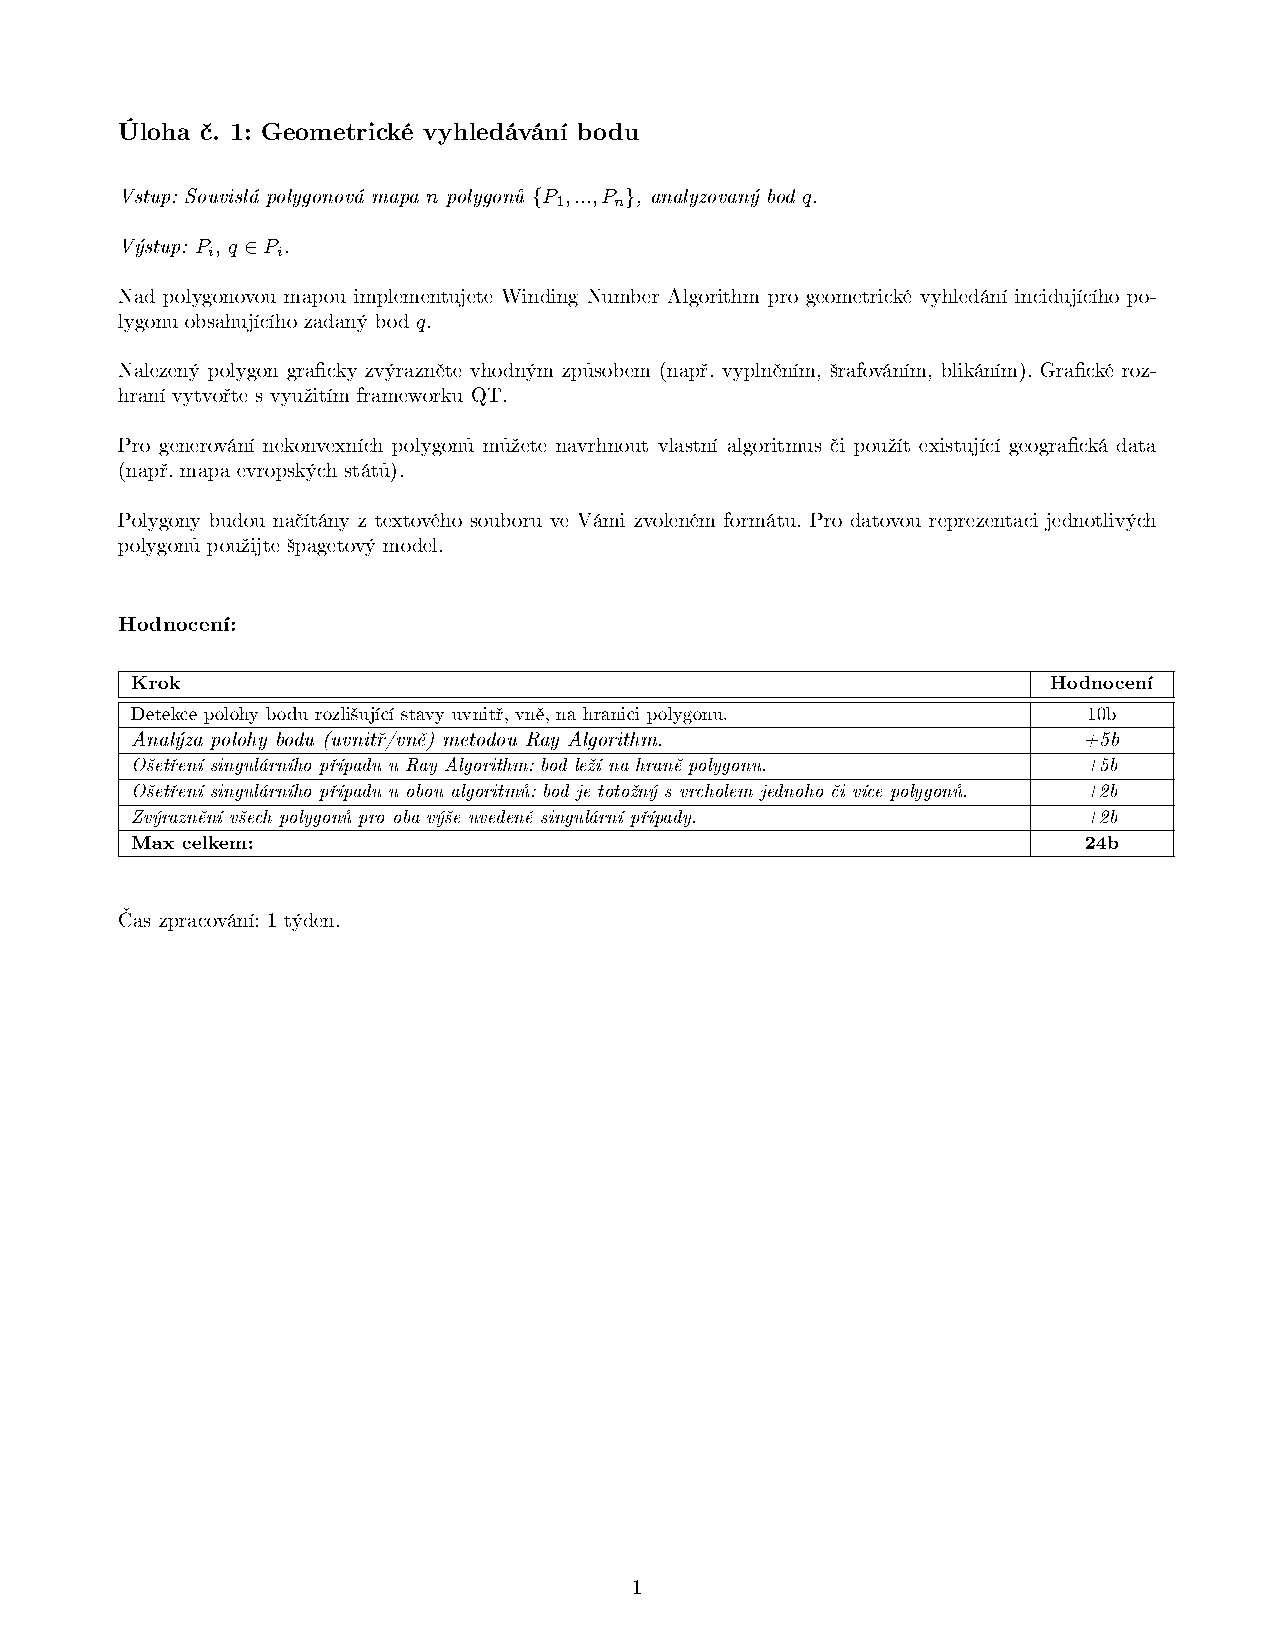
\includepdf{adkcv1}

%---------------------------------------------------------------------
\clearpage
\section*{Údaje o bonusových úlohách}
Bylo implementováno zjištění polohy bodu s využitím Ray Algorithm. Dále byly ošetřeny singularity v případech, kdy je určovaný bod totožný s vrcholem jednoho či více polygonů a pokud bod leží na hraně polygonu při řešení s užitím Ray Algorithm. 


\section*{Popis a rozbor problému}
% + vzorce
Nechť existuje polygon~$P$, který je tvořen jednotlivými vrcholy~$p_i$. V této úloze se konkrétně jedná o~načtený polygon (respektive více polygonů) se~souřadnicemi z~textového souboru ve~stanoveném formátu. Následně je nutné určit, zda~--~li je uživatelem zadaný bod~$q$ uvnitř, vně nebo na hranici polygonu. Vybraný polygon je graficky odlišen od ostatních. Výpočet polohy bodu vůči polygonu je popsán pomocí níže sepsaného postupu s~použitými vzorci.

Možné výsledky:
\begin{itemize}
\item Bod $q$ se nachází uvnitř polygonu~$P$.
\item Bod $q$ se nachází mimo polygon~$P$.
\item Bod $q$ leží na hraně polygonu~$P$.
\end{itemize}


\section*{Popisy algoritmů formálním jazykem}
\subsection*{Winding Number Algorithm}
Jestliže pozorovatel stojí na námi určeném bodě~$q$. Při určení polohy bodu vůči polygonu~$P$ se následně pozorovatel otáčí na bodě~$q$ proti směru hodinových ručiček. Při otočení proti směru hodinových ručiček, se úhlu přiřadí kladné znaménko a naopak, při otočení podél směru hodinových ručiček, je přiřazeno znaménko záporné. Pozorovatel takto zapisuje úhly~$\omega$ mezi jednotlivými vrcholy polygonu, dokud se nedostane do počátečního bodu. Dále se vypočte suma všech úhlů (tzv. Winding number) s~uvedením příslušných znamének a provede se určení polohy: 
\begin{itemize}
\item Pokud $q \in P$ a pozorovatel chce vidět více $\forall pi \in P$, musí se otočit o úhel 2$\pi$.
\item Pokud $q \notin P$, je tento úhel menší než 2$\pi$.
\end{itemize}


\noindent\textbf{Zadáno:} bod~$q$, polygon~$P$ tvořený vrcholy $p_i$

\noindent\textbf{Určováno:} úhly mezi vrcholy $\omega(p_i,q,p_{i+1} )$

\noindent\textbf{Implementace algoritmu:}

Ze souřadnic bodů jsou vypočteny vektory $\vec{u}_{\,i} = (q,p_i)$ a $\vec{v}_{\,i} = (q,p_{i+1})$. 

Dále probíhá výpočet jednotlivých úhlů: $\cos\omega = \dfrac{\vec{u}_{\,i}\cdot\vec{u}_{\,i}}{\vert\vec{u}_{\,i}\vert\cdot\vert\vec{v}_{\,i}\vert}$.

\begin{enumerate}
  \item Inicializace $\Omega = 0$, tolerance $\epsilon$. Natavení tolerance vychází z nutnosti porovnávání reálných, nikoliv celých, čísel.
  \item Opakování pro $\forall$ trojici $(p_i,q,p_{i+1} )$.
  \item \quad Určení polohy $q$ vzhledem k hranici polygonu $p = (p_i, p_{i+1})$. Tedy jestli bod leží vlevo, vpravo nebo na úsečce (hranici polygonu).
  \item \quad Určení úhlu $\omega_i = \angle p_i,q, p_{i+1}$.
  \item \quad Zjištění do jaké poloroviny bod patří. Pokud $q \in \overline{\Omega_l}$, pak $\Omega = \Omega + \omega_i$. Bod bude v ležet v levé polorovině.
  \item \quad Jinak $\Omega = \Omega - \omega_i$. Pak bod bude ležet v pravé polorovině. 
  \item Závěrem je proveden test na odchylku od $2\pi$. Pokud $\vert\vert\Omega\vert - 2\pi\vert < \epsilon$, pak se bod~$q$ nachází uvnitř polygonu~$P$.
  \item Jinak bod~$q$ leží mimo polygon~$P$.
\end{enumerate}


\subsection*{Ray Algorithm}
Bodem~$q$ je vedena polopřímka~$r$ (tedy paprsek, tzv. ray) ve směru osy~$X$. Jednotlivé průsečíky polopřímky~$r$ s~polygonem~$P$ jsou sčítány jen v~kladném nebo jen v~záporném směru osy~$X$. Jestliže je výsledný počet průsečíků lichý, pak bod~$q$ leží uvnitř polygonu~$P$. Jestliže je výsledný počet průsečíků sudý, pak bod~$q$ leží vně polygonu~$P$. 

Z~několika důvodů je vhodné použít upravenou variantu algoritmu s~redukcí ke~$q$. Mezi tyto důvody patří snadnější detekce hran protínajících~$r(q)$, jednodušší výpočet průsečíku~$M$, vyšší numerická stabilita a nezávislost na orientaci~$P$.\\

\noindent\textbf{Zadáno:} bod~$q$, polygon~$P$ tvořený vrcholy $p_i$

\noindent\textbf{Určováno:} počet průsečíků s polygonem~$P$

\noindent\textbf{Implementace algoritmu:}


\begin{enumerate}
  \item Inicializace $k = 0$. Počet průsečíků.
  \item Opakování pro $\forall$ body $p_i \in P$:
  \item \qquad $x^{'}_{i} = x_i - x_q$. Redukce x~--~ové souřadnice.
  \item \qquad $y^{'}_{i} = y_i - y_q$. Redukce y~--~ové souřadnice.
  \item \qquad Pokud $(y^{'}_{i} > 0)\&\&(y^{'}_{i-1} <= 0)\Vert(y^{'}_{i-1} > 0)\&\&(y^{'}_{i} <= 0)$.
  \item \qquad \qquad $x^{'}_{m} = \dfrac{x^{'}_{i} y^{'}_{i-1} - x^{'}_{i-1} y^{'}_{i}}{y^{'}_{i}-y^{'}_{i-1}}$
  \item \qquad \qquad Pokud $(x^{'}_{m} > 0)$, pak $k = k+1$.
  \item Pokud $(k\%2) \neq 0$, pak $q \in P$.
  \item Jinak $q \notin P$.
\end{enumerate}



\section*{Problematické situace a jejich rozbor}
% (tj. simplexy) + ošetření těchto situací v kódu
\subsection*{Winding Number Algorithm}
Tento algoritmus problematicky řeší případ, když je bod $q$ shodný s vrcholem polygonu~$p_i$.



\subsection*{Ray Algorithm}
Může nastat problém se singularitami, tudíž je vhodné použít upravenou variantu algoritmu, která je redukovaná k bodu $q$. Provede se tedy redukce do lokálního souřadnicového systému. 

\section*{Vstupní data}
% formát vstupních dat, popis
Vstupními daty jsou souřadnice jednotlivých polygonů, které se načítají do aplikace. Jedná se o textový soubor se třemi sloupci (ID bodu, $X$, $Y$) a tolika řádky, kolik je celkových bodů pro polygony. Souřadnice bodů jsou v lokálním souřadnicovém systému přímo pro aplikaci.


\section*{Výstupní data}
% formát výstupních dat, popis
Za výstup je považován výpis polohy bodu vůči polygonu v aplikaci a grafické znázornění bodu s polygony v okně aplikace. 

\section*{Snímky obrazovky vytvořené aplikace a její popis}
Po~zapnutí aplikace se~zobrazí prázdné okno pouze s~ikonami a výběrem algoritmu na~pravé straně (obr.~\ref{fig:app_zap_pol}). Stiskem tlačítka \emph{Load polygon} se otevře možnost vybrat textový soubor ve stanoveném formátu se souřadnicemi polygonů z~disku. Tímto je import polygonů hotov. 

\begin{figure}[htbh]
	\centering
	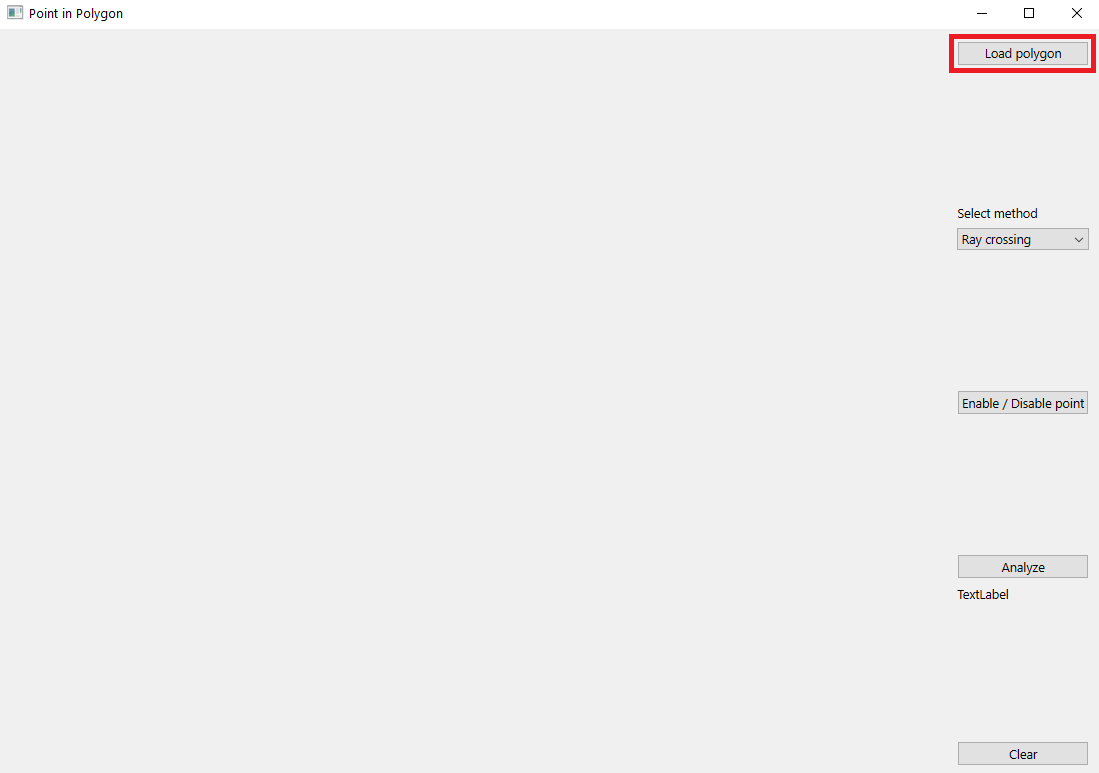
\includegraphics[scale=0.285]{obrazky/app_zapnuti.png}
	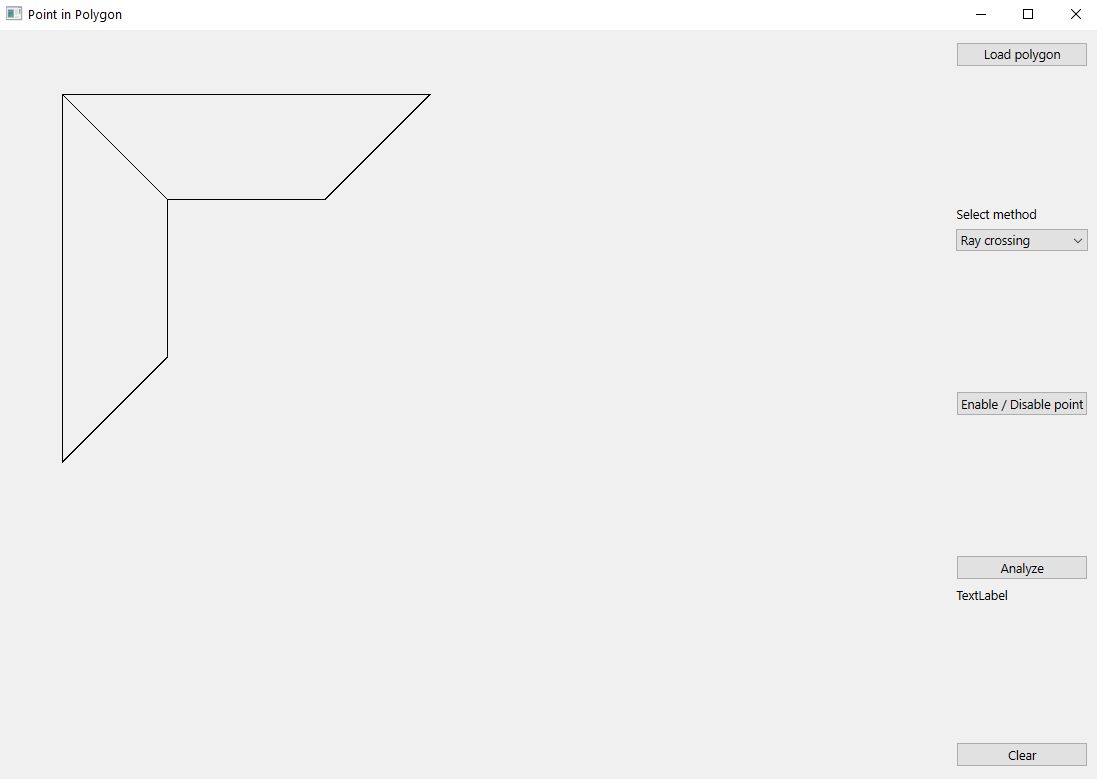
\includegraphics[scale=0.285]{obrazky/app_pol.png} 
	\caption{Aplikace po zapnutí (vlevo) a po načtení polygonů (vpravo).
	}
	\label{fig:app_zap_pol}
\end{figure} 
\FloatBarrier

Následně je potřeba stisknout tlačítko \emph{Enable/Disable point}, které umožňuje vkládání bodu do okna aplikace. Nyní je potřeba zvolit algoritmus pro určení polohy bodu přes otevření rozevírací nabídky pod názvem \emph{Select method} (obr.~\ref{fig:select_met}). Defaultním nastavením je Ray crossing algoritmus.

\begin{figure}[!htb]
	\centering
	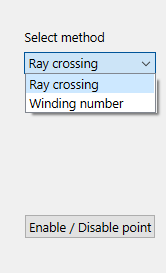
\includegraphics[scale=0.8]{obrazky/select_met.png} 
	\caption{Výběr algoritmu.
	}
	\label{fig:select_met}
\end{figure} 
\FloatBarrier

Pomocí tlačítka \emph{Analyze} je provedeno vyhodnocení výpočtu. Vpravo dole je vypsán výsledek. Možnosti jsou následující:
\begin{itemize}
\item \emph{Point is inside} $\longrightarrow$ Bod $q$ se nachází uvnitř polygonu~$P$.
\item \emph{Point is outside} $\longrightarrow$ Bod $q$ se nachází mimo polygon~$P$.
\item \emph{Point is on the border} $\longrightarrow$ Bod $q$ leží na hraně polygonu~$P$.
\end{itemize}

\begin{figure}[!htb]
	\centering
	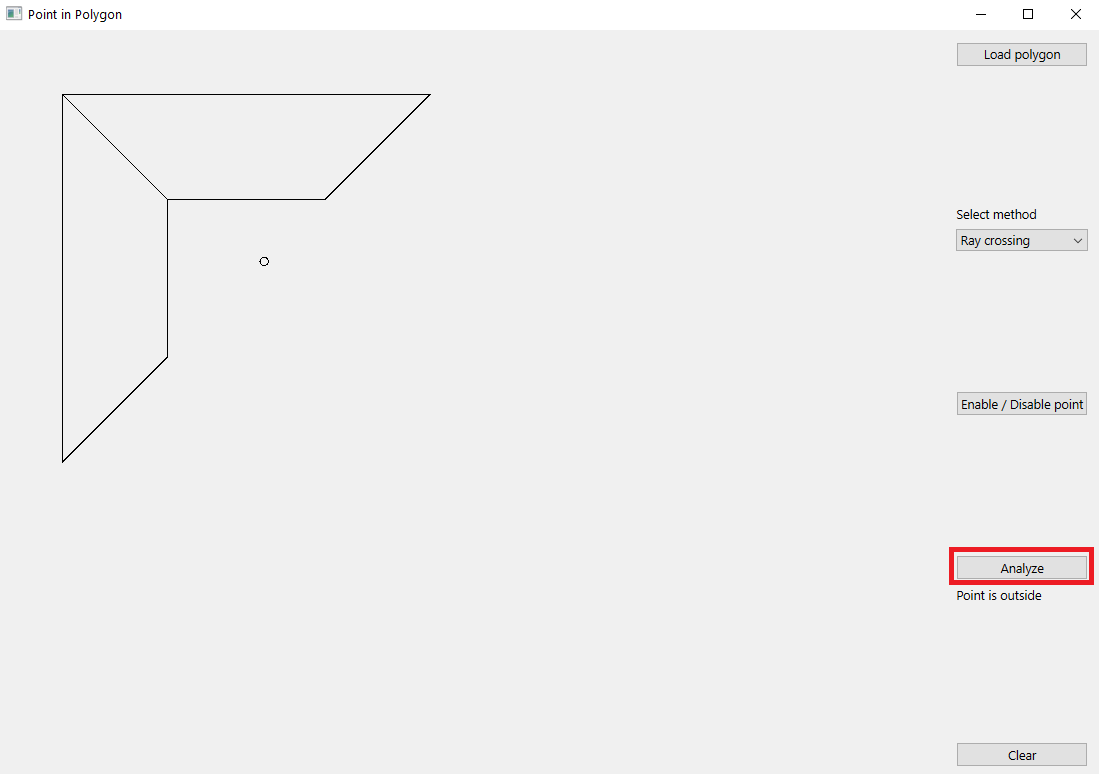
\includegraphics[scale=0.5]{obrazky/app_analyze.png} 
	\caption{Analýza polohy bodu vůči polygonu.
	}
	\label{fig:app_analyze}
\end{figure} 
\FloatBarrier

Při stisknutí tlačítka \emph{Clear} se provede vymazání všech načtených polygonů.

\section*{Dokumentace}
% popis tříd, datových položek a jednotlivých metod
\subsection*{Třída algorithms}
Tato třída obsahuje výpočetní vzorce pro použité algoritmy.

\textbf{Třída algorithms obsahuje následující veřejné metody:}
\begin{verbatim}
int getPointLinePosition(QPoint &a,QPoint &p1,QPoint &p2)
\end{verbatim}
Metoda určuje, zda~--~li bod leží v~levé či v~pravé polorovině od přímky (hrany polygonu). Vstupními parametry jsou určovaný bod~$a$ a body $p_1, p_2$, které tvoří přímku.\\

\begin{verbatim}
double get2LinesAngle(QPoint &p1, QPoint &p2, QPoint &p3, QPoint &p4)
\end{verbatim}
Metoda vypočte velikost úhlu, který svírají dvě přímky. První přímku tvoří body $p_1, p_2$ a druhou přímku body $p_3, p_4$.\\

\begin{verbatim}
int getPositionWinding(QPoint &q, std::vector<QPoint> &pol)
\end{verbatim}
Metoda určuje polohu bodu vůči polygonu za~pomocí algoritmu Winding Number. Vstupními parametry jsou souřadnice bodu~$q$ a souřadnice polygonů uložené ve vectoru~$pol$.\\

\begin{verbatim}
int getPositionRayCrossing(QPoint &q, std::vector<QPoint> &pol)
\end{verbatim}
Metoda určuje polohu bodu vůči polygonu za~pomocí algoritmu Ray Crossing. Vstupními parametry jsou souřadnice bodu~$q$ a souřadnice polygonů uložené ve vectoru~$pol$.

\subsection*{Třída draw}
Tato třída umožňuje vykreslování bodu a polygonů.

\textbf{Třída draw obsahuje následující privátní metody a proměnné:}
\begin{verbatim}
QPoint q
\end{verbatim}
Proměnná se souřadnicemi bodu~$q$, jehož poloha vůči polygonu je určována.\\

\begin{verbatim}
std::vector<QPolygon> polygons
\end{verbatim}
Proměnná, do které se ukládají načtené polygony z textového souboru.\\

\begin{verbatim}
bool enable_draw
\end{verbatim}
Proměnná, která povoluje vykreslování bodu.\\

\textbf{Třída draw obsahuje následující veřejné metody a proměnné:}
\begin{verbatim}
explicit Draw(QWidget *parent = nullptr)
\end{verbatim}
Prvotní vykreslení bodu~$q$ mimo okno aplikace.\\

\begin{verbatim}
void loadPolygon(std::string &path)
\end{verbatim}
Metoda, která načítá polygony z vybraného textového souboru na disku.\\

\begin{verbatim}
void paintEvent(QPaintEvent *event)
\end{verbatim}
Metoda, která vykresluje bod či polygony.\\

\begin{verbatim}
void mousePressEvent(QMouseEvent *event)
\end{verbatim}
Metoda určující souřadnice určeného bodu.\\

\begin{verbatim}
void clear()
\end{verbatim}
Metoda, která vymaže vybrané polygony z okna aplikace.\\

\begin{verbatim}
void changeStatus(){enable_draw = !enable_draw;}
\end{verbatim}
Metoda, která mění status kreslení bodu.\\

\begin{verbatim}
QPoint getPoint(){return q;}
\end{verbatim}
Vrací souřadnice bodu~$q$.\\

\begin{verbatim}
std::vector<QPolygon> getPolygons(){return polygons;}
\end{verbatim}
Vrací polygony při analyzování pozice.\\

\subsection*{Třída widget}
Tato třída propojuje uživatelské rozhraní aplikace s kódem. Je vytvořena v sekci \emph{Design}.

\textbf{Třída widget obsahuje následující privátní metody a proměnné:}
\begin{verbatim}
void on_pushButtonClear_clicked()
\end{verbatim}
Metoda, která určuje, co následuje po stisknutí tlačítka \emph{Clear}.\\

\begin{verbatim}
void on_pushButton_clicked()
\end{verbatim}
Metoda, která určuje, co následuje po stisknutí tlačítka \emph{Enable/Disable point}.\\

\begin{verbatim}
void on_pushButtonAnalyze_clicked()
\end{verbatim}
Metoda, která určuje, co následuje po stisknutí tlačítka \emph{Analyze}.\\

\begin{verbatim}
void on_pushButtonLoad_clicked()
\end{verbatim}
Metoda, která určuje, co následuje po stisknutí tlačítka \emph{Load}.\\


\section*{Závěr}
Cílem zadané úlohy bylo vytvoření aplikace, která uživateli umožňuje načíst souřadnice bodů z~textového souboru ve stanoveném formátu a následně určit, zda~--~li je uživatelem zadaný bod uvnitř, vně nebo na hranici polygonu. K výpočtu polohy bodu vůči polygonu byly použity dva algoritmy~--~Winding Numbers a Ray Crossing. Výsledná aplikace umožňuje načíst vlastní polygony a určit všechny tři výše zmíněné polohy bodu.

\subsection*{Možné či neřešené problémy}
Při situaci, ve které je bod součástí polygonu, není daný polygon graficky zobrazený. Jedná se o jednu z bonusových úloh.


\subsection*{Náměty na vylepšení}
Při zvolení bodu~$q$ totožně s~vrcholem polygonu by bylo možné vypsat samostatnou kategorii pro určení polohy (např. \emph{Point is on the vertex}). V tomto případě stávající program vypisuje hlášku \emph{Point is on the border}.

Použitý soubor s polygony slouží pouze pro ukázku, jistě by bylo možné jej dále rozvinout. 

Dále by bylo možné implementovat například nastavení přesnosti při určování nebo zápis souřadnic čísly namísto klikání myší.


\begin{flushright}
V Praze 18.10.2021\\
\vspace{2mm}
Bc. Pane Kuzmanov\\
Bc. František Mužík\\
\end{flushright}


\end{document}
